\documentclass[a4paper,12pt]{article}
\usepackage[fleqn]{amsmath}
\usepackage{amssymb}
\usepackage{graphicx}
\graphicspath{ {./images/} }
\begin{document}

\title{Calculus}	
\author{Edward Jex}
\maketitle
Calculus is the mathematics of change and has two distinct parts. Differentiation and Integration. 
\section*{Integration}
\begin{itemize}
	\item Rates of change
	\item Finding the gradient of a tangent to a curve at a point. 
\end{itemize}
\subsection*{Differentiating from First Principles}
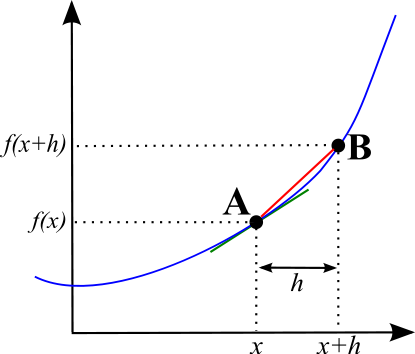
\includegraphics[scale=0.5]{Graph1}\\
The gradient of the tangent of the curve at A can be approximated by the gradient of the chord AB. As the distance h gets smaller, the approximation of the gradient gets better.  \\
$f'(a)$ - The gradient of the tangent to the curve $f(x)$ at $x=a$. \\
\begin{align*}
f'(A) & = \frac{f(B) - f(A)}{B - A} \\
& \simeq \frac{f(A+h) - f(A)}{h} \\
f'(a) & = \lim_{h \to 0} \frac{f(a+h) - f(a)}{h} \\
\end{align*}
\subsubsection*{Differentiating $y = x^2$ from First Principles}
\begin{align*}
f'(a) & = \lim_{h \to 0} \frac{(a + h)^2 - a^2}{h} \\
& = \lim_{h \to 0} \frac{a^2 + 2ah + h^2 - a^2}{h} \\
& = \lim_{h \to 0} 2a + h \\
& = 2a \\
\end{align*}
\subsection*{Tangents and Normals}
Tangent - Intersects the curve once locally. \\
Normal - Perpendicular to the tangent. \\ 
$m_1 \times m_2 = -1$ for perpendicular lines. \\ 
\subsection*{Stationary Points}
Stationary points are when $\frac{dy}{dx} = 0$. \\
Types:
\begin{itemize}
	\item Local minimum - Turning point and Stationary point
	\item Local maximum - Turning point and Stationary point
	\item Points of inflection - Stationary point
\end{itemize}
To tell which type of stationary point we have, we can look at the second derivative ($\frac{d^2y}{dx^"}$):
\begin{itemize}
	\item At a minimum - $\frac{d^2y}{dx^2} > 0$
	\item At a maximum - $\frac{d^2y}{dx^2} < 0$
	\item At a point of inflection - $\frac{d^2y}{dx^2} = 0$ 
\end{itemize}
If $\frac{d^2y}{dx^2} = 0$, the point could also be a turning point, more investigation is required. 
\subsection*{Shapes of Curves}
Points of infection ($\frac{d^2y}{dx^2} = 0$) have two types:
\begin{itemize}
	\item Stationary (where $\frac{dy}{dx} = 0$)
	\item Non-stationary
\end{itemize}
Points can be either concave up, concave down or points of infection. \\
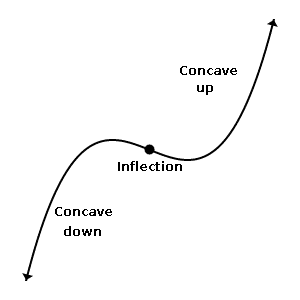
\includegraphics[scale=0.5]{Graph2} \\
\begin{itemize}
	\item Concave down - $\frac{d^2}{dx^2} < 0$, Cord is below the curve. 
	\item Concave up - $\frac{d^2}{dx^2} > 0$, Cord is above the curve.   
\end{itemize}
\subsection*{Optimisation}
Differentiation can be used to find minimum of maximum points for a problem which can be the optimum for given conditions. 
\section*{Differentiation Rules}
\subsection*{Trig Functions}
Note that these rules only work in radians. \\
\begin{tabular}{ c c }
\hline
	 $f(x)$ & $f'(x)$  \\ 
\hline
	$\sin f(x)$ & $f'(x) \cos f(x)$ \\
	$\cos f(x)$ & $-f'(x) \sin f(x)$ \\
	$\tan f(x)$ & $\frac{f'(x)}{\cos^2 f(x)} = f'(x)\sec^2 f(x)$ \\
\hline
\end{tabular}
\subsection*{Exponentials and Logarithms}
\begin{tabular}{ c c }
\hline
	 $f(x)$ & $f'(x)$  \\ 
\hline
	$a^{f(x)}$ & $f'(x) a^{f(x)} \ln a$ \\
	$\log_a f(x)$ & $\frac{f'(x)}{f(x)\ln a}$	 \\
\hline
\end{tabular}
\subsection*{Chain Rule}
Rates of change can be connected. We can calculate new rates of change by cancelling terms like fractions, although they are not fractions. $\frac{dy}{dx} = \frac{dy}{du} \times \frac{du}{dx}$. We also see fraction like behaviour when taking reciprocals as $\frac{dy}{dx} = \frac{1}{\frac{dx}{dy}}$. Note that you should not write this as $\frac{dx}{dy}^{-1}$. \\
The general rule is: $(f \circ g)' = (f' \circ g).g'$
\subsection*{Product Rule}
The general rule is: $(f.g)' = f'.g + f.g'$ \\
Note than sometimes an expression may be a fraction. You can treat the denominator as a negative power, or you could use the quotient rule. 
\subsubsection*{Quotient Rule}
The general rule is: $y = \frac{f}{g} \Rightarrow y' = \frac{f'.g - f.g'}{g^2}$. This can be easily derived from the product rule. I recommend always using the product rule because it is much nicer. 

\section*{Implicit Differentiation}
Implicit differentiation is used when there is no clear subject e.g. a circle. It relies on the principle than $\frac{d}{dx}f(y) = \frac{d}{dy}f(y) \times \frac{dy}{dx} = f'(y) \frac{dy}{dx}$.
\subsubsection*{Example 1}
\begin{align*}
x^2 + y^2 & = 25 \\
\frac{d}{dx}x^2 + \frac{d}{dx}y^2 & = \frac{d}{dx}25 \\
2x + 2y \frac{dy}{dx} & = 0 \\
\frac{dy}{dx} & = -\frac{x}{y} \\
\end{align*}
\end{document}